\section{Date: 2026-08-08}
\noindent \textbf{Series ID: CWUR0000SANL113} 

\noindent This series is titled Consumer Price Index for All Urban Wage Earners and Clerical Workers: Nondurables Less Food, Beverages, and Apparel in U.S. City Average and has a frequency of Monthly. The units are Index 1982-1984=100 and the seasonal adjustment is Not Seasonally Adjusted.The observation start date is 1967-01-01 and the observation end date is 2026-06-01.The popularity of this series is 1. \\ 

\noindent \textbf{Series ID: WSCNDW01FRA489N} 

\noindent This series is titled Work Started: Construction: Dwellings and Residential Buildings: Total for France and has a frequency of Annual. The units are Number, Monthly level and the seasonal adjustment is Not Seasonally Adjusted.The observation start date is 1960-01-01 and the observation end date is 2017-01-01.The popularity of this series is 1. \\ 

\subsection{Raw Regression}
\noindent Regresses the two series against each other directly. A significant result here can come just as easily from both series sharing a long-run trend as from any real relationship.

\begin{center}
\begin{tabular}{lclc}
\toprule
\textbf{Dep. Variable:}               & value\_fred\_WSCNDW01FRA489N & \textbf{  R-squared:         } &     0.048   \\
\textbf{Model:}                       &             OLS              & \textbf{  Adj. R-squared:    } &     0.028   \\
\textbf{Method:}                      &        Least Squares         & \textbf{  F-statistic:       } &     2.448   \\
\textbf{Date:}                        &       Sat, 08 Aug 2026       & \textbf{  Prob (F-statistic):} &    0.124    \\
\textbf{Time:}                        &           12:20:51           & \textbf{  Log-Likelihood:    } &   -517.37   \\
\textbf{No. Observations:}            &                51            & \textbf{  AIC:               } &     1039.   \\
\textbf{Df Residuals:}                &                49            & \textbf{  BIC:               } &     1043.   \\
\textbf{Df Model:}                    &                 1            & \textbf{                     } &             \\
\textbf{Covariance Type:}             &          nonrobust           & \textbf{                     } &             \\
\bottomrule
\end{tabular}
\begin{tabular}{lcccccc}
                                      & \textbf{coef} & \textbf{std err} & \textbf{t} & \textbf{P$> |$t$|$} & \textbf{[0.025} & \textbf{0.975]}  \\
\midrule
\textbf{const}                        &    3.398e+04  &     1785.119     &    19.035  &         0.000        &     3.04e+04    &     3.76e+04     \\
\textbf{value\_fred\_CWUR0000SANL113} &     -18.2426  &       11.660     &    -1.565  &         0.124        &      -41.674    &        5.189     \\
\bottomrule
\end{tabular}
\begin{tabular}{lclc}
\textbf{Omnibus:}       &  9.260 & \textbf{  Durbin-Watson:     } &    0.207  \\
\textbf{Prob(Omnibus):} &  0.010 & \textbf{  Jarque-Bera (JB):  } &    3.089  \\
\textbf{Skew:}          &  0.227 & \textbf{  Prob(JB):          } &    0.213  \\
\textbf{Kurtosis:}      &  1.883 & \textbf{  Cond. No.          } &     311.  \\
\bottomrule
\end{tabular}
%\caption{OLS Regression Results}
\end{center}

Notes: \newline
 [1] Standard Errors assume that the covariance matrix of the errors is correctly specified.

\begin{figure}
\centering
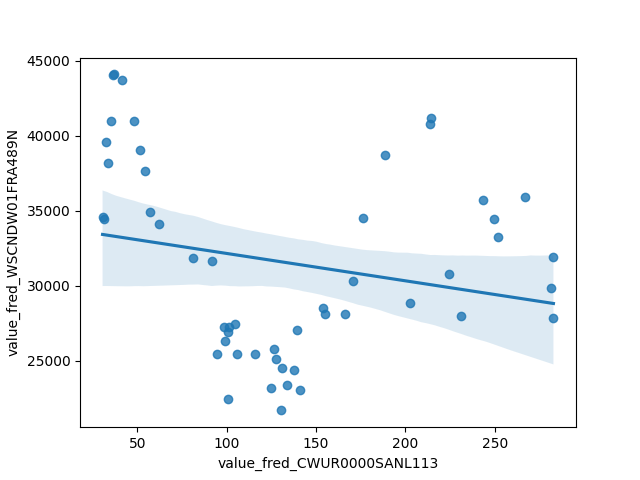
\includegraphics[scale = 0.9]{plots/plot_2026-08-08.png}
\caption{Raw Regression Plot for 2026-08-08}
\end{figure}
\newpage
\subsection{Detrended Regression}
\noindent Regresses the residuals of each series after removing its own linear time trend, so a shared trend can no longer drive the result on its own. A relationship that stays significant here is better evidence of a genuine link between the two series.

\begin{center}
\begin{tabular}{lclc}
\toprule
\textbf{Dep. Variable:}                          & value\_fred\_WSCNDW01FRA489N\_detrended & \textbf{  R-squared:         } &     0.082   \\
\textbf{Model:}                                  &                   OLS                   & \textbf{  Adj. R-squared:    } &     0.064   \\
\textbf{Method:}                                 &              Least Squares              & \textbf{  F-statistic:       } &     4.405   \\
\textbf{Date:}                                   &             Sat, 08 Aug 2026            & \textbf{  Prob (F-statistic):} &   0.0410    \\
\textbf{Time:}                                   &                 12:20:51                & \textbf{  Log-Likelihood:    } &   -514.05   \\
\textbf{No. Observations:}                       &                      51                 & \textbf{  AIC:               } &     1032.   \\
\textbf{Df Residuals:}                           &                      49                 & \textbf{  BIC:               } &     1036.   \\
\textbf{Df Model:}                               &                       1                 & \textbf{                     } &             \\
\textbf{Covariance Type:}                        &                nonrobust                & \textbf{                     } &             \\
\bottomrule
\end{tabular}
\begin{tabular}{lcccccc}
                                                 & \textbf{coef} & \textbf{std err} & \textbf{t} & \textbf{P$> |$t$|$} & \textbf{[0.025} & \textbf{0.975]}  \\
\midrule
\textbf{const}                                   &   -5.457e-11  &      824.380     & -6.62e-14  &         1.000        &    -1656.654    &     1656.654     \\
\textbf{value\_fred\_CWUR0000SANL113\_detrended} &      90.3527  &       43.049     &     2.099  &         0.041        &        3.843    &      176.863     \\
\bottomrule
\end{tabular}
\begin{tabular}{lclc}
\textbf{Omnibus:}       &  4.999 & \textbf{  Durbin-Watson:     } &    0.260  \\
\textbf{Prob(Omnibus):} &  0.082 & \textbf{  Jarque-Bera (JB):  } &    2.635  \\
\textbf{Skew:}          &  0.308 & \textbf{  Prob(JB):          } &    0.268  \\
\textbf{Kurtosis:}      &  2.073 & \textbf{  Cond. No.          } &     19.1  \\
\bottomrule
\end{tabular}
%\caption{OLS Regression Results}
\end{center}

Notes: \newline
 [1] Standard Errors assume that the covariance matrix of the errors is correctly specified.

\begin{figure}
\centering
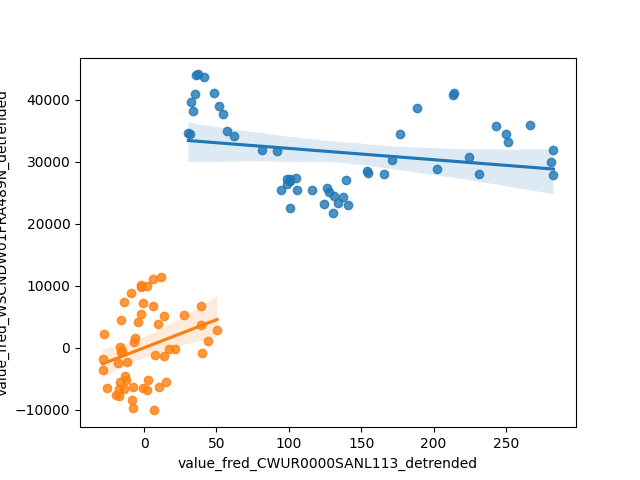
\includegraphics[scale = 0.9]{plots/plot_2026-08-08_detrended.png}
\caption{Detrended Regression Plot for 2026-08-08}
\end{figure}
\newpage
